389. В таблице $5\times5,$ клетки которой пронумерованы как на рисунке, необходимо отметить несколько клеток так, чтобы в каждой строке и в каждом столбце была отмечена ровно одна клетка. Кирилл отметил клетки с номерами 1, 13, 19 и ещё две. Чему может быть равна сумма номеров этих двух клеток?\\
\begin{figure}[ht!]
\center{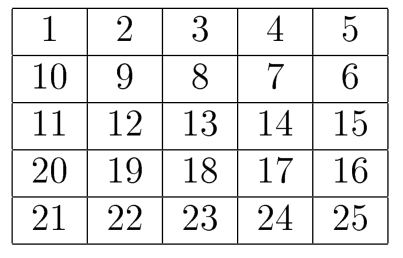
\includegraphics[scale=0.35]{tab5.png}}
\end{figure}\\
